% Reviderad 2024-10-08 emma strömberg


\documentclass{article}
\usepackage[utf8]{inputenc}
\usepackage[english]{babel}
\usepackage{amsmath}
\usepackage{listings}
\usepackage{graphicx}
\usepackage{comment}
\usepackage{float}
\usepackage{biblatex}
\usepackage{lscape}
\usepackage{csquotes}
\usepackage{multirow}
\usepackage{hyperref}
\usepackage{array} 
\usepackage{booktabs} 
\usepackage[a4paper,pdftex,bottom=20mm, width=160mm]{geometry}


\addbibresource{bibliography.bib}


\setlength{\parindent}{0pt}
\setlength{\parskip}{1em}

\title{
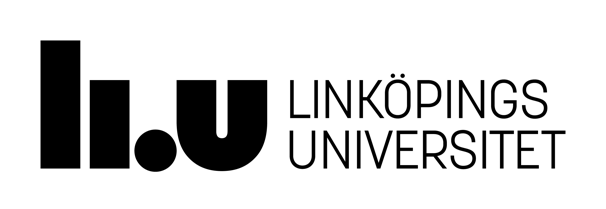
\includegraphics[scale=1.5]{liu_logga.png} \\
\vspace{2.0cm} \textbf{Software Quality Assurance Plan} \\
 \endgraf\rule{\textwidth}{.4pt}
  \large \textbf{TDDC88 - Project - Company 3}\\
}



\author{
% Add your full name here
    Emma Strömberg - Product and Sales Line Manager \and 
    Adrian Redfors - Technical Writer \and 
    Anton Hänström - Testing Lead \and 
    William Eriksson - Analysis Lead \and 
    Andreas Tetlie - Deployment Lead \and 
    Olle Lövborg - Process Manager \and 
    Chang Guo - Architecture
}
\date{\today}

\begin{document}

\begin{comment}

\section{Information for Authors}
Dear contributors to the Quality Assurance Plan,

Thank you for your participation in creating this document for our TDDC88 project. As we aim for grade 5, your input is vital to ensure a comprehensive and high-quality plan. Please note the following guidelines:
\begin{itemize}
    \item Deadline: The initial draft of your assigned section is due by [2024-10-4 \textit{may change}]. This allows time for review and integration before our next milestone. Note that not all parts f your section can be completed by this time. 
    
    \item Section Ownership: Your name has been assigned to a specific section. You are responsible for the content and timely completion of that section.
    
    \item Content Expectations: Aim for clarity and thoroughness. Each section should be approximately 300-500 words, but prioritize quality over quantity. Include specific, actionable details relevant to our project.
    
    \item Grade 5 Focus: We are aiming for grade 5. Ensure your section demonstrates:
    \begin{itemize}
        \item Integration with overall development processes
        \item Support for continuous improvement
        \item Forward-thinking approaches to quality assurance
    \end{itemize}
    
    \item Collaboration: While you're responsible for your section, feel free to consult with team members. 
    
    \item Version Control: Adrian will manage version control. Submit your updates in Overleaf by Wednesday evenings to be included in the weekly GitLab update.
    
    \item Questions: If you have any questions or need clarification, please contact Emma (Product and Sales Line Manager) or Adrian (Technical Writer).
\end{itemize}
Remember, this document is crucial for our project's success and our course grade. Your expertise and diligence are greatly appreciated.
Thank you for your commitment!
\textit{*Emma - Product and Sales Line Manager \& Adrian - Technical Writer}

\vspace{1cm}
\textbf{Sections and Responsible Authors:}
\begin{itemize}
    \item Document Structure and Ownership: \textit{Adrian TechnicalWriter}
    \item Testing Strategy: \textit{Anton TestingLead}
    \item Traceability: \textit{William AnalysisLead}
    \item Continuous Integration and Delivery: \textit{Andreas DeploymentLead}
    \item Bug Tracking and Resolution: \textit{Anton TestingLead}
    \item Internal Quality Practices: \textit{Olle ProcessManager}
    \item Change Management: \textit{*Olle* ProcessManager}
    \item Process Evaluation and Improvement: \textit{Emma ProductandSalesLineManager}
    \item Future Development and Operations: \textit{Chang Architecture}
    \item Implementation and Verification: \textit{Emma ProductandSalesLineManager}
\end{itemize}

\end{comment}

\maketitle

\newpage
```latex
\section{Document Change History}

\begin{center}
\small\textit{Note: This change history table was generated by Autoleaf AI under the supervision of the Technical Writer. Only the most significant changes are highlighted, check the readme.md, found in gitlab, for more detailed information.}

\vspace{0.5cm}

\begin{tabular}{|p{0.05\textwidth}|p{0.09\textwidth}|p{0.17\textwidth}|p{0.14\textwidth}|p{0.39\textwidth}|}
\hline
\textbf{Ver.} & \textbf{Date} & \textbf{Modified Areas} & \textbf{Changed By} & \textbf{Description of Changes} \\
\hline
2.2 & 2024-10-17 & Req. Struct., User Classes, Func. Req., Non-Func. Req., Design Constraints & Analyst Team & Restructure document for clarity and traceability, introduce sub-requirements linked to main requirements, rename and restructure user roles section. Remove Software System Attributes section. \\
\hline
2.1 & 2024-10-10 & User Stories, Scope, Non-Func. Req., Overall Desc. & Analyst Team & Restructure user stories, clarify scope, streamline non-functional requirement descriptions, and improve overall description clarity. \\
\hline
2.0 & 2024-10-03 & Software Sys. Attr., User Stories, Constraints, Assumptions, Func. Req., Perf. Req. & Analyst Team & Introduce software system attributes, refine user stories, expand constraints, clarify assumptions, and provide specific details for functional and performance requirements. \\
\hline
1.1 & 2024-09-24 & Intro, Overall Desc., Specific Req. & Analyst Team & Expand initial structure with detailed descriptions of user roles, system functionalities, requirements, and constraints. \\
\hline
1.0 & 2024-09-19 & Intro, Overall Desc., Specific Req., Supporting Info & Analyst Team & Establish initial structure and content of the Requirements Specification document. \\
\hline
\end{tabular}
\end{center}

\vspace{1cm}
```
 
\newpage


\tableofcontents
\newpage

\section{Introduction}
% \textit{Responsible: *Emma* ProductandSalesLineManager}
This Software Quality Assurance (SQA) Plan is a crucial document for our TDDC88 project, designed to ensure the highest quality standards in our software development process. Targeting a grade 5, this plan outlines the standards, practices, procedures, and tools our team will use to meet and exceed course requirements while delivering a product that is reliable, user-friendly, and meets the needs of our client. It details our testing strategies and defect management practices, establishing clear protocols to prevent, detect, and resolve issues efficiently. Through systematic quality control and improvement measures, we aim to minimize defects, maintain system stability, and optimize the user experience. Additionally, the SQA plan clarifies team roles and responsibilities in the quality process and outlines metrics and reporting mechanisms to track our progress. Adhering to these guidelines will enable us to achieve a product that is not only technically sound but also reflects the user-centric focus central to our client’s vision.

\subsection{Quality Objective}
In this project, usability is the primary quality factor guiding our software development and assurance processes. Our Analyst group has consulted extensively with the customer, Axis Communications, and together we have agreed that simplicity is key: fewer features and functions are preferred, as long as they work reliably and align closely with the specified requirements. Usability is essential because it directly impacts user satisfaction, productivity, and adoption rates. A highly usable product allows users to intuitively and efficiently accomplish their tasks without extensive training or frustration, meeting user needs while achieving business goals. By focusing on usability over extensive functionality, we aim to deliver a streamlined, dependable product that not only performs well technically but also integrates seamlessly into users' workflows, fostering trust and encouraging long-term engagement.

\subsection{Purpose}
This plan is designed to be a living document, regularly updated to reflect our evolving practices and lessons learned. Each section outlines specific quality assurance activities, their purpose, and the individuals responsible for their implementation.

The purpose of this document is twofold:
\begin{enumerate}
    \item To provide a comprehensive framework for maintaining and improving software quality throughout our development lifecycle.
    \item To clearly communicate responsibilities and expectations to all team members, ensuring a coordinated effort towards achieving our quality goals.
\end{enumerate}



\newpage
\section{Document Structure and Ownership}
% \textit{Responsible: *Adrian* TechnicalWriter}

This section details the overall structure of the SQA plan, ensuring it is well-organized, easily navigable, and accessible to all team members. The structure is designed to support continuous improvement and integration with our overall development processes.

\subsection{Document Structure}
The SQA plan is organized into clearly defined sections, each corresponding to a key aspect of our quality assurance process. This structure ensures:

\begin{itemize}
    \item Easy navigation and quick reference for team members
    \item Clear delineation of responsibilities
    \item Logical flow from high-level strategy to specific implementation details
    \item Facilitation of regular updates and continuous improvement
\end{itemize}

\subsection{Authorship}
Each section owner is responsible for authorship of their own section. This decentralized approach ensures that the content is created and maintained by those with the most relevant expertise. Responsibility for formatting and information sharing about the Quality Assurance plan is shared between Emma and Adrian:

\begin{itemize}
    \item \textit{Emma - Product and Sales Line Manager}: Responsible for stakeholder communication and ensuring alignment with project goals
    \item \textit{Adrian Technical Writer}: Responsible for version control, document formatting, and maintaining overall document consistency
\end{itemize}

This collaborative approach supports continuous improvement by leveraging diverse expertise and maintaining clear lines of communication. These include \textit{Lead Tester}, \textit{Lead Deployment}, \textit{Architect}, \textit{Lead Analyst}, and \textit{Process Manager}.

\subsection{Document Review}
All project documentation, including the SQA Plan, is subject to regular review by the \textit{Product and Sales Line Manager} to ensure it meets both internal quality standards and client expectations. This review process is a structured part of our document quality assurance approach explained in Section \ref{document_review}, aimed at identifying areas for improvement and ensuring alignment with project objectives and best practices.

\subsection{Version Control System}
To support requirements for integration with development processes and continuous improvement, we implement a robust version control system:

\begin{itemize}
    \item The document is primarily edited in Overleaf, a collaborative LaTeX editor, shared with all responsible authors
    \item Weekly updates are made to GitLab every Thursday at 8am, before the weekly company meeting
    \item Each GitLab update includes:
    \begin{itemize}
        \item The latest version of the document
        \item A brief note detailing changes made since the last update
        \item Any relevant discussion points or decisions made regarding the document
    \end{itemize}
    \item Special updates are made before tollgate meetings, taking precedence over the regular weekly schedule
    \item GitLab's version history feature is used to track changes over time, supporting our continuous improvement efforts
\end{itemize}

\subsection{Continuous Improvement and Integration}
This structure supports continuous improvement and integration with overall development processes by:

\begin{itemize}
    \item Enabling real-time collaboration through Overleaf
    \item Providing a clear schedule for updates, aligning with project milestones and meetings
    \item Utilizing GitLab's features to track changes and facilitate discussions
    \item Ensuring the SQA plan evolves alongside the project, reflecting current best practices and lessons learned
    \item Facilitating easy access and reference for all team members, promoting a culture of quality throughout the development process
\end{itemize}

It is our belief that by maintaining this structured approach to document management and version control, we ensure that our SQA plan remains a living, evolving guide that directly supports our commitment to high-quality software development and continuous process improvement.


\newpage
\section{Testing Strategy}
\textit{Responsible: *Anton* TestingLead}

\subsection{Testing Plan}
For Testing Plan and Process, see external document. \href{https://www.overleaf.com/project/66ff9154fca1f68722259739}{Click here to visit Testing Plan}


\subsubsection{Testing Tools}

\textbf{Git Pipeline:} \\
The Git pipeline is utilized for automating the testing process. It ensures that tests are executed automatically with each code modification, supporting continuous integration and reducing the need for manual testing.

\textbf{Microsoft Planner:}\\ 
Microsoft Planner is employed for logging and managing bugs. It provides a structured platform for tracking issues, assigning tasks, and monitoring progress, thus ensuring a more organized approach to the testing workflow.

\textbf{Generative AI:}\\
Generative AI is used to efficiently create a large volume of user tests. This allows for rapid generation of test cases, enhancing test coverage and accelerating the verification of the program’s functionality. In addition, it is anticipated that the automated generation of tests will increase their comprehensiveness and reduce biases that are more likely to occur when user tests are manually created by the testers.

\textbf{Requirement Traceability Matrix:} \\
The requirement traceability matrix links functional requirements to their corresponding tests and user stories. It facilitates tracking which tests should be applied at specific stages of development, while also documenting when tests are performed and whether they are successful.

\subsubsection{Strategy for Continuous Testing}

The continuous testing strategy is designed to ensure a seamless, high-quality development process that supports continuous delivery and integrates with other quality assurance (QA) processes. This approach is centered around automated testing, efficient issue tracking, and thorough requirement traceability, ensuring that defects are identified early and the system remains stable throughout its lifecycle.

\textbf{1. Automated Testing through Git Pipeline:}\\
At the core of the continuous testing strategy is the Git pipeline, which automates the execution of tests upon each code commit. This practice aligns with continuous delivery principles by enabling frequent and reliable code releases. Automated tests are triggered in real-time, ensuring that any integration issues are detected immediately. By doing so, the pipeline ensures a constant flow of feedback, allowing developers to address defects early in the development cycle and maintain a deployable state of the codebase at all times.

\textbf{2. Integration with Continuous Delivery:}\\
This testing strategy directly supports continuous delivery by ensuring that every piece of code is rigorously tested before it is merged into the main branch. The automated tests provide confidence that the code is ready for production deployment, reducing the risk of introducing bugs into the live environment. Furthermore, by automating regression testing, the strategy ensures that new features or updates do not disrupt existing functionality. This, combined with real-time feedback and early detection of issues, allows for shorter release cycles and faster delivery of updates to users.

\textbf{3. Bug Logging and Management with Microsoft Planner:}\\
Microsoft Planner is employed for comprehensive bug tracking and task management. Any issue detected during testing is logged into Planner, where it is categorized, prioritized, and assigned to developers for resolution. This tool provides transparency across the team and integrates with other QA processes such as code reviews, enabling developers to collaboratively address issues. Bug management in Planner ensures that no defect is overlooked, facilitating continuous improvement of the system's quality.

\textbf{4. Generative AI for Comprehensive Test Creation:}\\
Generative AI is utilized to automate the creation of extensive test cases, ensuring that tests cover a wide range of scenarios, including edge cases that may be overlooked in manual testing. This process mitigates human biases and provides a more objective evaluation of the system’s functionality. By producing a large number of test cases efficiently, the strategy supports continuous delivery by keeping up with the rapid pace of development and ensuring comprehensive coverage of the codebase as it evolves.

\textbf{5. Requirement Traceability Matrix for Test Management:}\\
The requirement traceability matrix plays a crucial role in connecting functional requirements with corresponding test cases and user stories. This matrix helps maintain alignment between the development progress and the testing activities. By tracking which tests are associated with which development milestones, it ensures that all requirements are tested thoroughly and at the appropriate stages. This also integrates with QA processes such as acceptance testing.

\textbf{6. Integration with Other Quality Assurance Processes:}\\

\begin{itemize}
    \item Description of testing tools to be used
    \item Process for reporting and analyzing test results
    \item Strategy for continuous testing throughout the development lifecycle
\end{itemize}

For grade 5, include how the testing strategy supports continuous delivery and how it integrates with other quality assurance processes.

\newpage
\section{Traceability}

Maintaining traceability between requirements, system design, and test documentation is crucial for ensuring the system development process is cohesive, verifiable, and aligned with project goals. This approach highlights the tools, processes, and benefits of traceability, including its role in supporting quality assurance and continuous improvement through out a project. Three key concepts in aiding traceability are version handling, the requirement traceability matrix and change management.

\subsection{Version Handling}
The project will utilize a Version Control System (VCS), specifically Git, to enhance traceability and streamline collaboration within the development team. Git will enable the tracking of changes in both source code and design documentation, providing a comprehensive history of modifications made throughout the project lifecycle. This functionality allows the team to document changes effectively, offering insights into who made specific alterations and when they occurred. By leveraging Git, the project gains accountability, as every commit includes metadata about the author and the purpose of the change. These commits can also aid communication and traceability through referencing requirements and user stories in commit messages. Furthermore version handling through the use of Git allows developers to use branching strategies to isolate work related to specific features, requirements or user stories. Once a feature is completed, it can be merged back into the main codebase, maintaining a detailed history of development efforts related to that requirement.

Some of the key advantages of this approach is supporting branching strategies to further enhance traceability by isolating work related to specific tasks, enabling referencing to requirements and user stories in commits and 

\subsection{Requirement Traceability Matrix}
To ensure that the project all project requirements are systematically addressed throughout the project lifecycle we will apply the use of a Requirement Traceability Matrix (RTM). The ambition is that mapping requirements to their corresponding deliverables, tests, and risks, will assist in maintaining a clear overview of project progress, provide transparency, enable accountability and ensures alignment with the project scope, discouraging scope creep.

A key advantage of a RTM is enabling bidirectional traceabilty, the ability to trace forward (e.g., from requirement to test case) and backward (e.g., from test case to requirement). This ensures all requirements are implemented and tested, preventing unnecessary features and assisting potential change management. 

\subsection{Change Management}
Change management could become crucial in this project as the the limited resources in terms of time means that development of the software must start before all requirements are set in stone in other to meet iteration deadlines. This in conjunction with the nature of software projects where changes to requirements are common due to evolving stakeholder needs, market shifts, or regulatory updates implies that a structured process of handling these changes in a controlled and efficient way could be of high value. When a change is requested, the RTM helps assess its impact by showing which parts of the system—requirements, code and test cases will be affected. This enables a clear understanding of the implications for project timelines, budgets, and risks.

\newpage
\section{Continuous Integration and Delivery}


\textbf{CI/CD contribution to the overall quality of the project}

Continuous Integration (CI) and Continuous Delivery (CD) are essential practices for modern programming projects because they streamline the development process, improve code quality, and ensure faster, more reliable releases. CI ensures that code changes are automatically tested and integrated into the main codebase frequently, preventing integration issues and reducing the chances of bugs accumulating. CD extends this by automating the deployment process, allowing for frequent, smaller updates to be delivered to production with minimal risk. Together, CI/CD promotes collaboration, improves developer productivity, and helps deliver high-quality software rapidly and consistently

\vspace{1em}
\textbf{CI/CD Pipeline Description}

Source Control (Git): The pipeline starts whenever a developer pushes code to the repository, triggering the continuous integration process.
Building Docker Images: The CI/CD pipeline will automatically build Docker images for each of the components (LAN Server, Front-End, and ACAP) when changes are made in the respective directories. The images are then pushed to a container registry like Azure Container Registry or Docker Hub.
Deployment to Kubernetes (AKS): After successful builds, the images are deployed to a Kubernetes cluster hosted in Azure. Kubernetes ensures that the containers are deployed in a scalable and resilient manner.
\vspace{1em}

\textbf{Tools used for automation}
\begin{itemize}
    \item \textbf{GitLab CI}: The platform manage the entire CI/CD process, from building Docker images to deploying them on Kubernetes.
    \item \textbf{Docker}: Docker is used to containerize the different components of your system, ensuring that they can run consistently across different environments.
    \item \textbf{Kubernetes}: Kubernetes is used to orchestrate the deployment and scaling of the Docker containers across a distributed environment, providing resilience and easy management of the services.
\end{itemize}
\vspace{1 em}

\textbf{Still not answered}
\begin{itemize}
    \item Integration with testing and other quality assurance processes
    \item Frequency of builds and deployments
\end{itemize}





\newpage
\section{Bug Tracking and Resolution}
\textit{Responsible: *Anton* TestingLead}

Outline the bug tracking system and processes:

\begin{itemize}
    \item Selected bug tracking tool
    \item Process for reporting, prioritizing, and assigning bugs
    \item Workflow for bug resolution and verification
    \item Metrics for tracking bug trends and resolution efficiency
\end{itemize}

For grade 5, describe how bug tracking data is used to drive continuous improvement in development practices.

\subsection{Selected bug tracking tool} 
Bugs will be tracked using the Microsoft Planner tool. This will be a way to track unexpected problems that come up in the project and have a way of managing them efficiently. This tool will be used to label the incidents in how important they are and in what order they will be handled. This is a way of tracking that will be efficient for development since Microsoft tools are used for more parts in the project. 


\subsection{Process for reporting, prioritizing, and assigning bugs}
The way that bugs will be reported is by creating an incident in Microsoft planner. After this is created the bug will be labeled by the creator on how important it is and how it should be prioritized. With Microsoft planner the team can create different boards for different types of bugs or label as severity. After this, for efficient communication, the scrum meetings will be used to discuss these incidents and who will be responsible for the resolution of the bug. This way every developer will have knowledge of the bug and a resolution can be discussed with the entire group. If bugs are not solved properly or other developers are not aware of the issue then that can cause more issues and unnecessary work.


\subsection{Workflow for bug resolution and verification}
The bug resolution will be solved in different ways depending on the issue, the developer, together with the team, will come up with a solution and the code will be fixed. After debugging, the member will merge the fixed code with the old code. The incident in Microsoft planner will be closed. The other developers can after that continue with their work in that code without being affected by the incident. 


\subsection{Metrics for tracking bug trends and resolution efficiency}
Tracking bug trends will be done manually from the incidents created in Microsoft planner when or if there is something that needs tracking. The aim for the project is that the debugging is done thoroughly so that there are no trends in bugs to track. If needed,  the tracking of trends will be done in excel. The Microsoft planner board that need analysis and tracking of trends will be exported into excel. There the developers can see trends in metrics and analyze the data. 


\subsection{Bug tracking for continuous improvement}
Bug tracking is important for continuous improvements as this allows the team of developers to see and understand the issues that has been raised and how they have been resolved. This means that if this issue comes up again there will be a quick resolution, but perhaps the issue will never come up again as the team knows what to avoid. The bug tracking enforces this when the group of developers discuss this during the scrum-meetings and have this communications on bugs and debugging.



\newpage
\section{Internal Review Practices}
Internal review practices are fundamental to ensuring the quality and success of our project. By embedding these practices into our workflows, we make quality and routine procedures integral to every aspect of our work.

To support these routines without introducing unnecessary bureaucratic steps, we will use effective tools for collaboration, communication, document management, and code repositories. Communication channels, such as chat groups in Teams, are used to keep everyone informed about ongoing quality initiatives and any urgent quality issues. During internal meetings, participants are encouraged to continuously evaluate quality-related matters. The goal is to make quality work an integrated part of our daily workflow.

\subsection{Document Quality Assurance}
\label{document_review}
To achieve this, we are introducing a system for continuous review of critical documents, in the form of code changes, design specifications, test plans, and reports. Project members are encouraged to work iteratively with documents and other tasks to promote continuous improvement of what is delivered both internally and externally. Work will also go through continuous review, with different members at various stages taking on the roles of both author and reviewer. This ensures that different perspectives are applied to each part of the work. These principles aim to identify potential problems early and promote knowledge sharing.

Each review consists of a thorough assessment of the document's clarity, completeness, technical accuracy, and compliance with project requirements. Following the review, the reviewer provides detailed feedback to the relevant document author(s), including specific recommendations or required changes. The assigned authors are then responsible for incorporating this feedback promptly, with additional follow-up reviews scheduled as needed to confirm the updates. This iterative process helps maintain high documentation quality throughout the project life-cycle and ensures that all materials remain current, comprehensive, and valuable to project stakeholders. 

\subsection{External Meeting Quality Assurance}
Before each important external meeting, such as the tollgate meeting, thorough internal reviews, or walkthroughs, will be conducted. These sessions will involve the company to examine upcoming deliverables in detail and verify that they meet our established quality standards and align with the project goals. Any deviations or areas for improvement identified during these reviews are addressed immediately, ensuring that what is presented to external stakeholders meets the standards we strive for within the project.



\newpage
\section{Change Management}

The need for changes arises in most situations and is an integral part of the project. The processes within the project related to handling changes are designed to be agile and minimally bureaucratic. This allows for quick adaptation to new information and requirements while maintaining high-quality standards.

Team members are encouraged to continuously reflect on and identify areas where efficiencies or other changes need to be made. This can include functional changes, new requirements, or adjustments to processes. When a need for improvement is identified, it should be communicated within the team. This can be done in various forums depending on the nature of the requested change, such as digital internal communication channels and meetings. In this context, a brief description of the change, the reason for the proposed change, and the expected effects should be presented.

An analysis is then conducted in collaboration with relevant team members like developers, testers, and the Process Manager. The analysis evaluates potential effects on the project’s scope, timeline, resources, and quality. To keep the process efficient, we focus on key factors and avoid excessive documentation. A discussion then takes place within the team, and depending on the nature of the change, decisions are made according to existing organizational principles. At this stage, the person expected to make the decision about the change is involved. Approval of changes occurs as close to the change as possible. This can be within a cross-functional team or a working group. However, larger changes should be anchored with relevant line managers, the Process Manager, or the Project Manager.

The outcome is quickly shared with the team for transparency and is rapidly integrated into the project’s work. All affected documentation—such as requirement specifications, design specifications, and test plans—is updated according to what the decided change requires. We ensure clear communication of changes through information during team meetings and, when necessary, in digital communication channels. This aims to keep all team members informed and aware of their responsibilities related to the change.

\newpage
\section{Process Evaluation and Improvement}
The following chapter contains a presentation of the processes for evaluating and improving the company's practices to ensure that quality is maintained. Included is a description of the evaluation and a schedule of each evaluation session, metrics for measuring process effectiveness, a description of the procedure for implementing and documenting improvements, and lastly an overview of the feedback loop all company employees can use to give continuous feedback and recommendations to the quality assurance practices that are employed. 

\subsection{Schedule and Method for Regular Evaluation of QA Processes}
\label{schedule_and_method_for_regular_evaluation_of_qa_processes}
The project contains one pre-study and four iterations. After each iteration there will be a demo of the progress the company has made, as well as a sprint retrospective evaluating the practices of the company for the previous iteration and a sprint planning session for the upcoming iteration. The dates for each sprint and each sprint retrospective can be found in Table \ref{tab:iteration_table}. 

% Dates for retrospectives to be updated
\begin{table}[H]
    \centering
    \caption{Overview of iterations and dates for sprint retrospective}
    \begin{tabular}{|c|c|c|c|}
    \hline
        \textbf{Iteration} & \textbf{Start} & \textbf{End} & \textbf{Sprint Retrospective}\\\hline
        Pre-Study & 2024-09-13 & 2024-09-26 & n.d. \\\hline
        It.1 & 2024-09-30 & 2024-10-11 & 2024-10-17 \\\hline
        It.2 & 2024-10-14 & 2024-11-08 & \\\hline
        It.3 & 2024-11-11 & 2024-11-22 & \\\hline
        It.4 & 2024-11-25 & 2024-12-06 & \\\hline
    \end{tabular}
    \label{tab:iteration_table}
\end{table}

During the retrospectives, an overall assessment of practices during the previous iteration will be conducted. The Line Managers will collect feedback from each Lead and encourage each employee to utilize the feedback loop. The gathered information will be given to the Process Manager, who will summarize it into an overall evaluation. This will ensure continuous assessment of quality related practices.


\subsection{Feedback Loops from Team Members and Stakeholders}
To ensure consistent assurance of quality within all practices of the company, all employees are encouraged to contact their Lead, Line Manager, or the Project Manager to address their concerns and/or suggestions. Depending on the scope of the feedback, a Lead could act independently or raise the issue to their Line Manager. The Line Managers and the Project Manager will raise the issue to the manager group.

External stakeholders to the company may also raise quality assurance issues to the company. The most prominent stakeholder for this is the supervisor for Requirements, Testing, Configuration Management and Quality: Torvald Mårtensson. His feedback will be given during supervisor meetings on Thursdays or through e-mails to the Product and Sales Line Manager, who will act accordingly and inform the manager group. Any other external stakeholder is encouraged to give their feedback to any of the managers through teams, face-to-face meetings, or e-mail as they see most convenient. 

\subsection{Metrics for Measuring Process Effectiveness}
\label{metrics_for_measuring_process_effectiveness}
% Emma continue writing 


\subsection{Procedure for Implementing and Documenting Improvements}
All issues, regarding processes and procedures regarding quality, brought to the attention of the manager group, either through the evaluation process or feedback loops, will be documented, assessed, and if it affects a large part of the company it will be brought up on the following weekly meeting. 

The evaluation will be documented through the process described in Section \ref{schedule_and_method_for_regular_evaluation_of_qa_processes}. Issues from the feedback loops will be included in the \textit{Evaluation Report}, yet it will additionally be addressed immediately. This means that it will be included in the \textit{Weekly Status Report}. The assessment will be done through the \textit{metrics for measuring process effectiveness} described in Section \ref{metrics_for_measuring_process_effectiveness}. The response to each issue is dependent on the consequences of the issue. However, implementation will be introduced by a post in the appropriate teams-channel or in front of the entire company at the weekly meetings on Thursdays. 


\newpage
\section{Future Development and Operations}
\textit{Responsible: *Chang* Architecture}

This section outlines critical strategies and methodologies to prepare the system for future growth, covering both technical and operational aspects. Scalability, long-term support, and adaptability are key pillars of our future development roadmap. Below, we explore the necessary architectural adjustments, ongoing maintenance plans, and evolving quality assurance practices that will be instrumental in achieving sustainable scalability and operational excellence.

\subsection{Architectural Considerations for Future Scalability}

As our system grows, it’s crucial that the architecture scales efficiently, both in terms of handling more users and increasing system complexity. Several considerations and improvements can be made:

\begin{itemize}
    \item \textbf{Kubernetes Deployment}: By transitioning the \textit{External Server} to a \textit{Kubernetes cluster}, we gain \textit{automatic scaling}, \textit{load balancing}, and \textit{self-healing} capabilities. Kubernetes will enable us to automatically scale services up or down based on load, ensuring the system performs optimally under different conditions.
    \item \textbf{Microservices Architecture}: While we currently operate with more monolithic structures in each of our servers, moving to a \textit{microservices architecture} would improve scalability. This means breaking down services (like alarm management, scheduling, user authentication) into smaller, independently scalable components.
    \item \textbf{Message Queuing}: Implementing a \textit{message queue} (e.g., \textit{RabbitMQ} or \textit{Kafka}) for managing alarms and device requests ensures that the system can handle sudden spikes in alarms or user requests without overwhelming the servers.
\end{itemize}

\subsection{Plans for Long-Term Maintenance and Support}

For long-term maintenance, we need clear strategies for maintaining the system and ensuring it can evolve with minimal disruptions:

\begin{itemize}
    \item \textbf{Modular Codebase}: The system’s code should be modular, allowing individual parts to be updated, refactored, or replaced without affecting the whole system. This makes it easier to add new features, handle bug fixes, or introduce optimizations over time.
    \item \textbf{Monitoring and Alerts}: Implement comprehensive \textit{monitoring and alerting} to track system health, detect bottlenecks, and address issues proactively. Logs and performance metrics should be continuously analyzed to foresee potential failures.
    \item \textbf{Documentation and Knowledge Sharing}: Maintain thorough \textit{documentation} for the codebase, APIs, and infrastructure. Regular knowledge-sharing sessions between developers can help new team members onboard quickly and reduce reliance on key individuals.
\end{itemize}

\subsection{Strategies for Adapting QA Processes as the Project Evolves}

As the project grows, adapting our \textit{Quality Assurance (QA)} processes is essential to maintain the system’s reliability and performance:

\begin{itemize}
    \item \textbf{CI/CD Pipelines}: Continuous Integration and Continuous Deployment (\textit{CI/CD}) pipelines should be implemented to automate testing and deployment, reducing manual intervention. This ensures that updates are rolled out efficiently, with minimal downtime.
    \item \textbf{Performance Testing}: As we scale, \textit{performance and stress testing} become essential to ensure that the system can handle increasing loads, especially for live video streaming and alarm processing. Tools like \textit{Locust} or \textit{K6} can simulate large numbers of users and devices to test system behavior under load.
    \item \textbf{Test Coverage and Code Quality}: Regularly track \textit{test coverage} using libraries like \textit{Coverage.py} to ensure that a high percentage of the code is tested. Integrate linting tools like \textit{Ruff} into our CI/CD pipeline to ensure consistent style and coding standards.
    \item \textbf{Security Audits}: Regularly perform \textit{security audits} to identify vulnerabilities, particularly given the system's handling of sensitive data (such as alarms and video clips). Incorporating manual \textit{code review} sessions along with static analysis tools like \textit{Bandit} can help ensure the security of the system during these audits.
\end{itemize}


This forward-looking section is essential for grade 5, showing consideration of the project's long-term quality needs.

\newpage
\section{Implementation and Verification}
In the following chapter a plan for roll-out of the Software Quality Assurance (SQA) plan will be determined. Training of employees, cross-checks against course and project grading criteria, and approach to external and internal reviews are also presented below. 

\subsection{Roll-out and Training Plan}
Rolling out the SQA plan to the team requires a well-structured approach to ensure smooth adoption and alignment with project goals. The first step is a presentation of the purpose and scope of the SQA plan with the entire company, led by the Project Manager, Process Manager and Product and Sales Line Manager. Thereafter, each employee who's role is directly affected by the quality assurance plan will be introduced to and have expectations clarified during their startup meeting with the Product and Sales Line Manager. During these meeting, responsibility of writing certain parts of the plan and ensuring its execution is distributed. Following this, detailed documentation, including the plan itself, will be shared via the project's collaborative platforms Teams, Overleaf, and GitLab. An accessible version history, will help ensure that the company remains informed and aligned with the plan's expectations throughout the project's lifecycle.

To further support this rollout, training or orientation sessions are critical. These sessions, led by section owners or subject-matter experts, should cover each major component of the QA plan. For instance, the Testing Lead could conduct a session on the testing strategy, while the Process Manager might focus on internal QA practices and the importance of continuous improvement. These sessions ensure that each team member understands not only the QA tools and processes but also how their work directly impacts software quality. Regular attendance is important, with the training materials made available on the shared platform for future reference.

\subsection{Cross-check to Grading Criteria}
Regular cross-checks against course grading criteria help ensure that the project remains aligned with the requirements necessary for achieving a high grade. During these cross-checks, led by the Process Manager or Technical Writer, the company will review current progress and documentation, assessing whether all outlined QA processes are being adhered to. These assessments will be compared with the course's grading rubric, specified on the TDDC88-website and the grading criteria excel owned by the Process Manager, to identify any gaps or areas requiring additional focus. Regular check-ins will help maintain a high standard of work, ensuring that every section of the SQA plan meets academic and project standards.

\subsection{External and Internal Feedback}
Periodic reviews with supervisors are another critical step in maintaining alignment with external expectations. The supervisor for Quality Assurance, Testing, and Configuration would provide valuable feedback on how well the company's processes align with both the course goals and industry best practices. These reviews will be included in the weekly supervisor meetings, ensuring that feedback is consistent. It will also be incorporated into the company’s sprint retrospectives and process evaluations.

Finally, internal audits of QA practices ensure ongoing compliance with the plan. The Process Manager, alongside Line Managers and Leads, will conduct these audits, reviewing the team's adherence to internal processes like document versioning, bug tracking, and code reviews. These audits, scheduled in the sprint retrospectives, will help ensure that all activities are both proactive and in line with the overarching goals of the project. 

\newpage
\section{Conclusion}
This SQA Plan provides a comprehensive framework for ensuring high-quality software development in our TDDC88 project. By following this plan and continuously improving our processes, we aim to deliver a superior product while meeting all requirements for grade 5 in the course.

All team members are expected to familiarize themselves with this plan and actively contribute to its implementation. Regular reviews and updates will ensure that our quality assurance practices remain effective and aligned with project goals throughout the development lifecycle.

\end{document}